\begin{figure}
    \begin{subfigure}{.5\textwidth}
    
    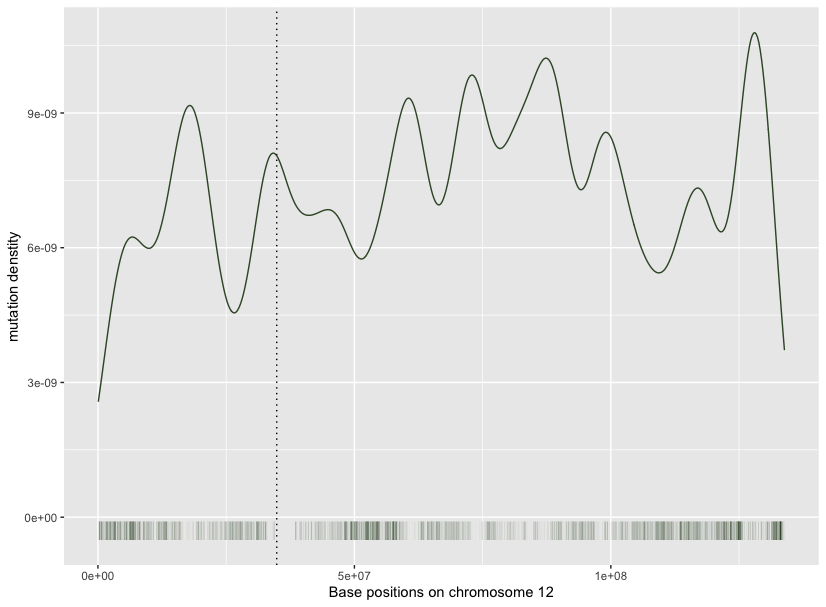
\includegraphics[width=\linewidth,height=0.7\textwidth]{graphics/mutdistribution_melanoma.png}
    \caption{Skin-Melanoma}
    \label{fig:density_skin}
    \end{subfigure}
    ~
    \begin{subfigure}{.5\textwidth}
    
    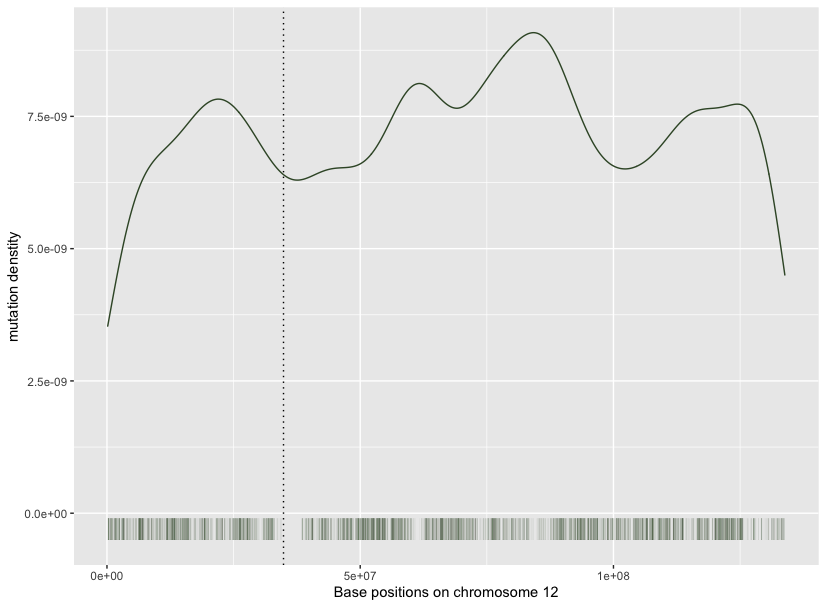
\includegraphics[width=\linewidth,height=0.7\textwidth]{graphics/mutdistribution_kidney.png}
    \caption{Kidney-RCC}
    \label{fig:density_kidney}
    \end{subfigure} \\
    
    \begin{subfigure}{.5\textwidth}
    
    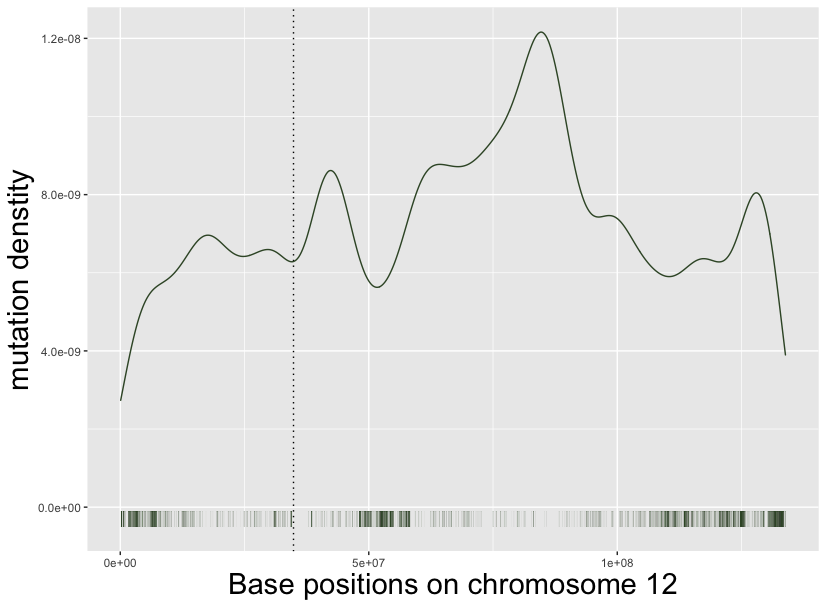
\includegraphics[width=\linewidth,height=0.7\textwidth]{graphics/mutdistribution_Liver-HCC.png}
    \caption{Liver-HCC}
    \label{fig:density_liver}
    \end{subfigure}
    ~
    \begin{subfigure}{.5\textwidth}
    
    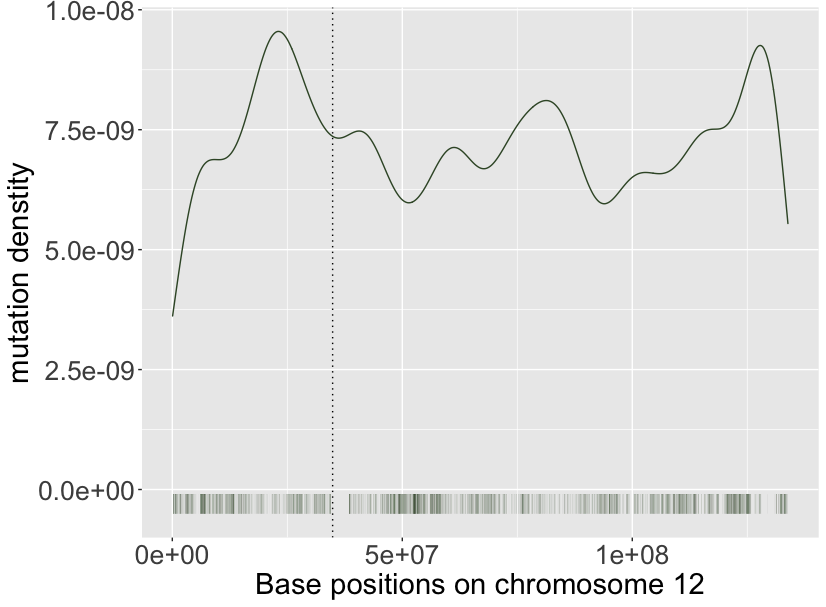
\includegraphics[width=\linewidth,height=0.7\textwidth]{graphics/mutdistribution_Panc-AdenoCA.png}
    \caption{Panc-AdenoCA}
    \label{fig:density_panc_adenoca}
    \end{subfigure} \\
    
    \caption{\textbf{Density}. The x-axis indicates the original base of a SBS, the y-axis indicates the base that it is mutated to. The height of a letter at a SBS is the $RE$ value for that SBS. If the letter is upside down, there is a decrease of abundance when moving from the first to the second cancer and vice versa.}
    \label{fig:mutation_density}
\end{figure}